\documentclass[12pt]{article}
\usepackage{textcomp}
\usepackage{cmap}				    	% поиск в PDF
\usepackage{mathtext} 	           
\usepackage[T2A]{fontenc}			% кодировка
\usepackage[utf8]{inputenc}			% кодировка исходного текста
\usepackage[english]{babel}
\usepackage[colorlinks=true,urlcolor=darkgray,citecolor=darkgray,linkcolor=darkgray,bookmarks=true]{hyperref}
% \usepackage{ccaption}
\usepackage{authblk}
\usepackage{indentfirst}
% \usepackage{float} 
\usepackage{amsmath}
\usepackage{apacite}
\usepackage{natbib}
\usepackage{graphicx}
\usepackage{comment}
\usepackage{amsfonts}
\usepackage{bm}
\usepackage{amssymb}
\usepackage{amsthm}
\usepackage{mathtools}
\usepackage{upgreek} % AMS
\usepackage{marvosym}
\usepackage{threeparttable}
\usepackage{etoolbox}
\usepackage{cmap}	
\usepackage{multirow}
\usepackage{fullpage} 
\usepackage{geometry}
\geometry{
 a4paper,
 total={210mm,297mm},
 left=20mm,
 right=20mm,
 top=20mm,
 bottom=20mm,
 }
\usepackage{url}
\usepackage{pgfplots}
\usepackage{caption}
\usepackage{longtable}
\usepackage{multirow}
\usepackage{booktabs}
\usepackage{makecell}

\usepackage{pgf}
\usepackage{tikz}
\pgfplotsset{compat=1.15}
\usepackage{mathrsfs}
\usepackage{tikz} 
\usepackage{pgfplots}
\usepackage{pgfplotstable}
\usepackage{braket}
% \usepackage[capposition=top]{floatrow}
\usepackage{verbatim}
% \usepackage[position=bottom]{subfig}
\usepackage{graphicx}
%\usefonttheme[onlymath]{serif}
\usepackage[colorinlistoftodos]{todonotes}
\usepackage{setspace}% Интерлиньяж
\onehalfspacing % Интерлиньяж 1.5
%\doublespacing % Интерлиньяж 2
%\singlespacing % Интерлиньяж 1
\usepackage{econometrics}


\usepackage{appendix}



\usepackage{hyperref}
\usepackage{varioref}
\usepackage{cleveref}
\usepackage{fancyref}

\usepackage{csquotes} 



\usetikzlibrary{arrows}
\usetikzlibrary{calc}
\usetikzlibrary{positioning}
\usetikzlibrary{fit}
\usetikzlibrary{backgrounds}
\usetikzlibrary{intersections}
\tikzset{
style1/.style={
line cap=round,line join=round,
axis/.style={thick, ->, >=stealth'},
l/.style={thin},
d/.style={dashed, thin}, 
pile/.style={thin, <->, >=stealth',shorten <=3pt, shorten >=3pt}, 
every node/.style={color=black}, 
}
}





% \usepackage[backend=biber,
% style=chicago-authordate]{biblatex}
% \addbibresource{references.bib}

 \def\references{\bibliography{references.bib}
 \bibliographystyle{econ}}



\usepackage{parskip}

\setlength{\parindent}{15pt}
\setlength{\parskip}{5pt}

% \renewcommand{\maketitle}{\begin{center}
%         \noindent{\bfseries\scshape\Large\@title} 
%         \noindent{ \itshape\large\card{\subtitle}} 
%         \par  \vspace{0.5ex}
%         \noindent {\large\itshape\@author}
%         \noindent{\card{\footnotesize \itshape \extratext}}
%         \end{center}
%         } 

    % \makeatother
    % \def\extratext{}
    % \def\topic{}
    % \def\subtitle{}
       
 \newcommand{\card}[1]{ \ifthenelse{\equal{#1}{}}{}{ {\par#1}}}

 \usepackage{lipsum}

 \makeatletter
 \def\blfootnote{\gdef\@thefnmark{$\dagger$}\@footnotetext}
 \makeatother




    %%% Работа с картинками
    \usepackage{graphicx}  % Для вставки рисунков
    \setlength\fboxsep{3pt} % Отступ рамки \fbox{} от рисунка
    \setlength\fboxrule{1pt} % Толщина линий рамки \fbox{}
    \usepackage{wrapfig} % Обтекание рисунков текстом
    \usepackage{rotating}%поворот figure


    \DeclareRobustCommand{\firstsecond}[2]{#1}


    \makeatletter
\newcommand\footnoteref[1]{\protected@xdef\@thefnmark{\ref{#1}}\@footnotemark}
\makeatother


\usepackage{rotating}
% \usepackage{caption}
\usepackage{subcaption}
\captionsetup{labelfont=bf, labelsep=period, skip=0pt}


\pagestyle{plain}

\title{Influence of Executive Power on the Judiciary. Court Chairman}
\author{Alexander I. Vlasov\thanks{Email: avlasov(at)nes.ru. I would like to thank To Be Precise project and Andrew Sudarkin for their work on increasing courts transparency; and \citet{R,tidyverse,Spark,sparklyr,Stargazer,plm} for statistical packages.}}
\date{\normalsize First version: November 1, 2023\\\vspace{1ex} This version: November 1, 2023\\ \vspace{1ex}
\href{https:}{Click here for the most recent draft} }
\numberwithin{equation}{section}
\numberwithin{table}{section}
\numberwithin{figure}{section}
\begin{document}
\maketitle


% \begin{abstract}
%     \noindent 123\\
%     \vspace{-1ex}\\
%     % \noindent\textbf{Keywords:} 123\\
%     % \vspace{-1ex}\\
%     \noindent\textbf{JEL Codes:} D72, K40 \\
%     \bigskip
% \end{abstract}


This paper explores the influence of court chairman on judicial decisions in criminal proceedings by exploring changes in their veto-power over judicial candidates appointment. 
In 2018 the State Duma of Russia passed a federal law which changed the process of judges appointments. 
This plausibly exogenous change in court chairman's power presents a rare example of a partial reduction in control of executive powers, that comes through the chairman, over the individual judges' decisions.

To examine the effect of the policy on verdicts I collect the data on all verdicts that were made in Russia between 2014 and 2022 and examine the judge-level and court-level influence on the cross-section of judicial decisions.

The degree of executive branch control over the judges cannot be directly observed.\footnote{Except in special circumstances as in \citet{Mcmillan2004}.} 
In this work I use  the approach similar to \citet{Mehmood2022}, i.e. the variation in judicial appointment procedure in order to identify the causal effect of reduction in executive power influence. 
Only a few studies have been investigating the judiciary in autocratic and weak democratic countries. 
My work investigates the role of court chairman (which represent the influence of executive power) in the contexts of Russian courts and the impact of a change of their powers on verdicts.

This work also relates to the broader topic of the importance of the courts as checks and balances to the executive powers and their role in economic development, such as \citet{North1990,Acemoglu2001,LaPorta2004,Rodrik2004}. 

I also relate to the general branch of work exploring the judiciary systems.
Most of the literature on judiciary is focused on examining influence of gender, racial and religious and biases they cause in the behavior of judges such as \citet{Alesina2014, Mehmood2023}.


\section{Background}

Formally the chairman\footnote{Sometimes legal literature refers to court chairman as ``court presidents'' as in, for example, \citet{Zholobov2022}.} of the court is one of the judges who is entrusted with duties that are necessary for the court functioning. 
The chairman is vested primarily with organizational powers, most of which relate to the work of the court apparatus, rather than the work of judges. 
But in daily practice a court chairman turns out to be the chief mechanism of informal control in the judicial system \citep{Makarova2017}. 

Further I describe the mechanisms through which a court chairman can exercise their control over the judges as of before the September 2019, the change that has happened is described in \vref{subsection:243}.

\subsection{Court Chairman's Powers}




First of all, a court chairman has an influence on the judge hiring process. 
A court chairman is responsible for reporting that there is a vacant position of a judge to a qualification board of judges, and in case of disagreement with the board's decision, the chairman of the court is able to turn the proposed candidate for reconsideration. 
This is effectively constitutes a veto power over any judge appointment in the particular court the chairman presides. 

Another mechanism of the power of the chairman is the distribution of cases among the judges of the court they preside. 
There is no legislation that restricts methods and criteria for the distribution of cases among judges.
In rare cases, courts use the techniques of random distribution, but, as a rule, the case for a particular judge is assigned by the chairman of the court.\footnote{The main issue with a widespread adoption of systems random case distribution is technical limitations and shortage of funds \citep{Galkina2019}.}

The chairman of the court can use its discretionary right of cases distribution to influence the outcome of the proceeding. 
\citet{Makarova2017} notes that there have been instances when court chairmen, in order to obtain the decision they needed, entrusted those to judges from whom they have expected the desired decision. 
Additionally to judge distribution, all of the  organizational and management decisions are made by the chairman of the court. 
These include coming up with a vacation schedule, the technical equipment of the workplace and the number and qualifications of assistants and secretaries for a particular judge. 
So, a court chairman theoretically is able either choose a judge that will make a desired decision, or coerce a judge into making the decision by a threat of deterioration of working conditions and other inconveniences.\footnote{See \citet{Zholobov2022} (in English) for a detailed review of court chairman powers, responsibilities, and regulatory acts.}


This system makes ordinary judges highly dependent on the chairman of the court they work in; the chairmen of the courts themselves are dependent on the chairmen of higher-level courts; and they, in turn, on the President of the Russian Federation, who appoints them.
Also, the power concentration in the hands on court chairman lead to a greater possibility of court corruption and influence from the executive power \citep{Zholobov2022}.  
Note that the executive power interests (prosecutor's office and investigative bodies) is that every case that is brought to court is won and the requested sentence is granted. 



\subsection{Federal Law 243 2018 (243-ФЗ 2018)}
\label{subsection:243}

The legislation from june 29th, 2018 (243-ФЗ, henceforth)\footnote{243-ФЗ or 243-FZ (reeds like ``Fe Ze'')  stands for 243 Federal Law which is passed by the State Duma (bicameral federal parament of Russia) in 2018-07-29.} that was enacted on the 1st of september, 2019 the chairman of a court does no longer hold a veto power over the judge candidacy. 
After the 243-ФЗ enactment the chairman of the court can no longer refuse a recommendation of the qualification board on the judge appointment. 
The same law has also abolished the right of the chairman to apply to the qualification board of judges with a statement to bring the judge to disciplinary action \citep{Koroleva2021}.
Although a court chairman has retained the main mechanism of influence on judges (through the distribution of court cases), the control over the hiring process is supposed to be reduced by this law. 


\subsection{Influence of Executive Power on Judges}


\section{Data}

My empirical analysis uses data of all of the criminal verdicts for almost all regions in Russia which came from the ``Justice state information system'' which I further refer to by its url name SUDRF.\footnote{In Russian: Государственная автоматизированная система Российской Федерации <<Правосудие>>. It can be accessed via \url{sudrf.ru}.} 
It was launched in November 30, 2006 and the system hasn't had a major engine update since then, what makes it hard to interact with. 
In order to solve the issue of slow access, To Be Precise and Andrew Sudarkin has made SUDRFScraper, which automates web-scrapping from the SUDRF.

For some of the regions data is not available. 
Particularly, currently it is not possible to obtain any data from any of the annexed regions,\footnote{That are Republic of Crimea, Sevastopol, Donetsk People's Republic, Luhansk People's Republic, Zaporizhzhia Oblast, Kherson Oblast.} Chechnya, and Tver Oblast. 
In all of the regions mentioned, except Tver Oblast, the probable cause for absence of data is the overall lack of transparency of regional powers caused by hostilities and (at least partial) rule of military administrations. 
There is no particular reason why Tver Oblast's servers are not accessible. 
Also, I need to note that the number of cases in Ingushetia is suspiciously small, what makes the results in this region not reliable, so it was omitted. 

The full dataset is comprised of court verdict observations from 80 (at the point of writing I've collected 53) regions from 2015-01-01 to 2022-01-01. \footnote{There are $83$ regions (federal subjects) in Russian Federation in 2015-01-01/2022-01-01. Tver Oblast, Chechnya and Ingushetia are omitted. }
I restrict the observations to this time period from the above due to potential influence of change in the regime from informational autocracy (spin dictatorship) towards repressive regime (fear autocracy)\footnote{See \citet{GurievTreisman2020} for definitions and in-depth theoretic discussion and \citet{GurievTreisman2022} for more casual discussions.} that happened with a start of Russian invasion of Ukraine on 24 February 2022, what can constitute a structural change in the judicial process. 
Restriction from below is done so the treatment (243-ФЗ) is relatively centered in the dataset timespan.

In \vref{Summary:1} you can see the summary statistics describing all of the verdicts that were made from 2015-01-01 to 2022-01-01 as they are presented in the SUDRF database. 


I randomly sample 30,000 observations from this large dataset after the variable creation stage in order to ease calculations of inference for each of the regression I make. 


\subsection{Outcome Variables}

I restrict the sample described in \vref{Summary:1} to two first types of decisions: ``A verdict was made'' and ``The criminal case has been terminated'' since other types of decisions by a court are more complex and they will be harder to work with in aggregate data. 
This two categories of decisions covers more than 93\% of the overall sample


Note, that the verdicts as they are classified in SUDRF, are quite general (``A verdict was made'' do not give us any information on what a particular verdict was) and for finer distinction I'm parsing the texts of decisions\footnote{Specifically, I parse the final part, called court statement -- ``постановление суда.''} in search of the specific words indicating type of decision.  
The first 
This variable is codified only for those observations that I was able to obtain texts.
I classify all of the ``A verdict was made'' decisions into the following categories: Guilty, Prison, and Suspended. 
``Guilty'' is a dummy variable indicating whether the indictee was found guilty. 
``Prison'' is a dummy variable that indicates whether the prison was the outcome of the court proceedings.
``Suspended'' indicates whether the prison sentence was suspended.

I need to note that it is not the most accurate way of construction, specifically compared with \citet{Mehmood2022,LaPorta2008,Djankov2003}, who ask law firms to code the outcome variables. 
Approach I choose, on the other hand, allows me to widen the considered samples at no dollar cost, but probably with lower accuracy.

In order to examine the decisions of the judges hired after the 243-ФЗ reform in full, I construct the set of Verdict, Guilty, Prison, and Suspended variables for the nonrestricted sub-sample as well as for subsamples of particular charges based on penal code -- those are homicide (article 105 of criminal code), fraud (article 156) and drugs possession (article 228).\footnote{The full name of the article 228 is: ``Illegal acquisition, storage, transportation, production, processing of narcotic drugs, psychotropic substances or their analogues, as well as illegal acquisition, storage, transportation of plants containing narcotic drugs or psychotropic substances, or their parts containing narcotic drugs or psychotropic substances.''}

The additional differentiation into specific crimes give us insight on what was the particular effect of 243-ФЗ reform on the cross-section of the verdicts. 
Homicides suppose to represent violent crimes, fraud represents economic crimes and drugs possession represents the crimes against society. 
Those are the most populous representors of the aforementioned categories.


\begin{table}[!htbp]\centering\scriptsize
    \begin{threeparttable}
    \caption{Number of Cases per Decision. 2015--2020}
    \label{Summary:1}
    \begin{tabular}{@{\extracolsep{3pt}}lc} 
        \\[-1.8ex]\hline 
        \hline \\[-1.8ex] 
    \thead{Decision} &\thead{Number of cases\\ (Share of sample)} \\ \hline \\
    \makecell[l]{0. Number of observations} & \makecell[c]{1,534,546\\ (100\%)}\\ & \\
    \makecell[l]{1. A VERDICT was made} &  \makecell[c]{1,210,757 \\ (78.9\%)}  \\ \\[-1.8ex] 
    \makecell[l]{\quad 1.1 Guilty} &   \makecell[c]{919,891\\ (60.0\%)}  \\ & \\
    \makecell[l]{\qquad 1.1.1 Prison} &   \makecell[c]{357,058\\ (23.3\%)}  \\ & \\
    \makecell[l]{\qquad 1.1.2 Suspended sentence} &   \makecell[c]{324,801\\ (21.2\%)}  \\ & \\
    \makecell[l]{\qquad 1.1.3 Other} &   \makecell[c]{238,032\\ (15.5\%)}  \\ & \\
    \makecell[l]{\quad 1.2 Other} &   \makecell[c]{290,866\\ (18.9\%)}  \\ & \\
    \makecell[l]{2. The criminal case\\\quad has been TERMINATED}  &\makecell[c]{218,282 \\ (14.2\%)} \\ & \\
    3. Another decision was made & \makecell[c]{40,917\\ (2.67\%)}  \\ & \\
    \makecell[l]{4. Sent to appropriate\\\quad JURISDICTION} &     \makecell[c]{19,411\\(1.26\%)}  \\&\\
    \makecell[l]{5. COMPULSORY MEDICAL \\\quad MEASURES applied} & \makecell[c]{16,706 \\ (1.09\%)}  \\&\\
 
    \makecell[l]{6. RETURNED TO THE \\\quad PROSECUTOR}  & \makecell[c]{16,640 \\ (1.08\%)} \\&\\
    \makecell[l]{7. REFUSED to accept \\\quad the application for legal \\\quad proceedings}  &\makecell[c]{5,641\\ (0.37\%) } \\&\\
    \makecell[l]{8. Appeal PROCEEDINGS IS\\\quad  TERMINATED}& \makecell[c]{2,088\\(0.14\%)}  \\&\\
    9. NA & \makecell[c]{1,942\\ (0.13\%)}  \\&\\
    \makecell[l]{10. WITHDRAWN from appeal\\\quad consideration} &   \makecell[c]{1,227 \\ (0.08\%)}\\&\\
    \makecell[l]{11. Submission (complaint)\\\quad is WITHDRAWN} &   \makecell[c]{499\\ (0.03\%)} \\&\\
    \makecell[l]{12. Case joined to another case} &  \makecell[c]{479\\ (0.03\%)}  \\&\\
    \makecell[l]{13. LEFT WITHOUT \\\quad CONSIDERATION due to  \\\quad non-appearance of the parties}&\makecell[c]{29\\ (0.00\%)} \\  \\[-1.8ex]\hline 
    \hline \\[-1.8ex] 
    \end{tabular}
    \begin{tablenotes}[flushleft]
        \item[] \textit{Notes}: This table presents number of cases and their share conditional on verdicts in the full sample. The main categories are coded in SUDRF. The subcategories are derived from texts of decisions.
    \end{tablenotes}
\end{threeparttable}
    \end{table}



\begin{table}[!htbp] \centering \footnotesize
    \begin{threeparttable}
    \caption{Descriptive Statistics on Variables Used} 
    \label{} 
  \begin{tabular}{@{\extracolsep{7pt}}lccccc} 
  \\[-1.8ex]\hline 
  \hline \\[-1.8ex] 
  Variable & \multicolumn{1}{c}{Observations} & \multicolumn{1}{c}{Mean} & \multicolumn{1}{c}{SD} & \multicolumn{1}{c}{Min} & \multicolumn{1}{c}{Max} \\ 
  \hline \\[-1.8ex] \multicolumn{5}{l}{\textit{Panel A: All Articles}} \\ \\[-1.8ex] 
  Verdict & 30,000 & 0.848 & 0.359 & 0 & 1 \\ 
  Guilty & 24,067 & 0.804 & 0.397 & 0 & 1 \\ 
  Prison & 24,067 & 0.316 & 0.465 & 0 & 1 \\ 
  Suspended & 24,067 & 0.281 & 0.450 & 0 & 1 \\  \\[-1.8ex] 
  Treated & 30,000 & 0.051 & 0.220 & 0 & 1 \\ 
    Share of new & 30,000 & 0.052 & 0.129 & 0 & 1 \\ 
    Post & 30,000 & 0.324 & 0.468 & 0 & 1 \\  \\[-1.8ex] 
  \makecell[l]{Number of Letters \\ \quad  (thousands)}&  22,723 & 18.861 & 39.381 & 0 & 3,151.7 \\ 
  Instance $=$ First & 30,000 & 0.798 & 0.402 & 0 & 1 \\ \\
  \multicolumn{5}{l}{\textit{Panel B: Homicide -- Article 105}} \\ \\[-1.8ex] 
  Verdict & 24,061 & 0.984 & 0.127 & 0 & 1 \\ 
Guilty & 18,219 & 0.972 & 0.166 & 0 & 1 \\ 
Prison & 18,219 & 0.804 & 0.397 & 0 & 1 \\ 
Suspended & 18,219 & 0.051 & 0.221 & 0 & 1 \\  \\[-1.8ex] 
Treated & 24,061 & 0.036 & 0.188 & 0 & 1 \\ 
Share of new & 24,061 & 0.048 & 0.110 & 0 & 1 \\ 
Post & 24,061 & 0.254 & 0.435 & 0 & 1 \\  \\[-1.8ex] 
  \makecell[l]{Number of Letters \\ \quad  (thousands)} & 18,067 & 42.813 & 33.020 & 0.000 & 1,788.0 \\ 
  Instance $=$ First & 24,061 & 0.770 & 0.421 & 0 & 1  \\ \\
  \multicolumn{5}{l}{\textit{Panel C: Fraud -- Article 159}} \\ \\[-1.8ex] 
  Verdict & 30,000 & 0.798 & 0.401 & 0 & 1 \\ 
  Guilty & 24,906 & 0.748 & 0.434 & 0 & 1 \\ 
  Prison & 24,906 & 0.262 & 0.440 & 0 & 1 \\ 
  Suspended & 24,906 & 0.330 & 0.470 & 0 & 1 \\ \\[-1.8ex] 
  Treated & 30,000 & 0.044 & 0.206 & 0 & 1 \\ 
 Share of new & 30,000& 0.048 & 0.115 & 0 & 1 \\ 
Post & 30,000 & 0.313 & 0.464 & 0 & 1 \\ \\[-1.8ex] 
  Number of letters &23,543 & 43.323 & 101.141 & 0.000 & 5,741.1 \\ 
  Instance $=$ First & 30,000 & 0.842 & 0.365 & 0 & 1 \\
  \\
  \multicolumn{5}{l}{\textit{Panel D: Drugs -- Article 228}} \\ \\[-1.8ex] 
  Verdict & 30,000 & 0.978 & 0.146 & 0 & 1 \\ 
  Guilty & 25,457 & 0.970 & 0.169 & 0 & 1 \\ 
  Prison & 25,457 & 0.373 & 0.484 & 0 & 1 \\ 
  Suspended & 25,457 & 0.361 & 0.480 & 0 & 1 \\  \\[-1.8ex] 
  Treated & 30,000 & 0.042 & 0.200 & 0 & 1 \\ 
  Share of new & 30,000 & 0.048 & 0.122 & 0 & 1 \\ 
  Post & 30,000 & 0.262 & 0.440 & 0 & 1 \\  \\[-1.8ex] 
Number of letters & 25,294 & 20.579 & 33.555 & 0.000 & 1,405.7\\ 
Instance $=$ First & 30,000 & 0.879 & 0.326 & 0 & 1 \\   
\\[-1.8ex]\hline \hline
  \end{tabular} 
  \begin{tablenotes}[flushleft]
    \item[] \textit{Notes}: This table reports the summary statistics for the 4 samples used in regressions in Main results.
  \end{tablenotes}
\end{threeparttable}
  \end{table} 

\subsection{Main Explanatory Variables}
\label{sec:MainExplonatory}
A key explanatory variable used in the analysis is $\textit{Treated}_{j,r,t}$. It is a dummy variable indicating whether a particular judge precising over a case was hired before or after the change in hiring practice (243-ФЗ) was implemented. 
Since we are not able to determine the particular date of the hiring, I deduce it from the date of the first verdict a particular judge have made, it is expected to happen within a weak after a hiring. 


Note that the judge that was hired after september the 1st, 2019 (after the 243-ФЗ was enacted) was not subjected to a veto of court chairman.  
What is more important, this treatment will be enacted independently of court chairman since they do not influence the availability of vacant jobs, which is capped on yearly basis by the federal budget.

Additionally, to measure the aggregate effect of treatment, that is, with an inclusion of potential spillovers from treated judges to untreated judges in the same court, I construct the variable $\textit{Share of New}_{crt}$ which is defined as a share of treated (hired after 2019-09-01) judges in a court $c$. 

\subsection{Control Variables}

Since we do not observe judge characteristics (except their names),\footnote{Note that since the text of judicial decisions are in Russian language, it is possible to determine gender of judge and indictees only from their names with high accuracy. But it is rather laborious task, so I leave it for further possible improvements.} we can control only for characteristics of the case. 
I control for length of the verdict (in thousands of characters) and instance (first or appeal). 
I combine this controls with twoways region-year fixed effects in each of the specification.



\section{Empirical Methodology}

\subsection{Effect of Treatment}



The first specification I use is the regression of outcome variables 
\begin{equation}
    Y_{ijcrt}=\alpha\, \textit{Treated}_{jcrt}+X_{ijcrt}'\gamma+\tau_{rt}+\varepsilon_{cjrt},\label{eq:treat}
\end{equation}
where indexing is done as follows $i$, $j$, $c$, $r$, $t$ index case, judge, court, region (federal subjects), and year, respectively. Vector $X_{ijcrt}$ is a vector of control variables, it include length of the verdict and instance (first or appeal).

As described in previously, the the treatment variable, $\textit{Treated}_{j,r,t}$, is equal to one if judge $j$ was hired after $j$. 
To achieve causal interpretation (by relying on credible conditional independence) we need to assume that treatment and outcomes are independent conditional on the vector of controls and fixed effects. 
This assumes away the situations where a potential judge decides to become one due to (at least partially) the Federal Law 243 (243-ФЗ).
That is, we need to assume that there is no selection bias caused by not conditioning on some of the characteristic of a judge.\footnote{This assumption is essentially that we can perfectly predict the decision of a given judge by the controls, i.e. the post-conditioning residual variance and outcome variable (decision) are independent.}
And since the nature of the dataset I have obtained does not allow me to account for a rich set of characteristics of a judge (unlike \citet{Mehmood2022}), the CIA in this case seems to be a non-credible assumption. 
This means that the coefficient on the $\textit{Treated}_{j,r,t}$ variable can only be interpreted as noncausal.



To adjust for clustering I use double-clustered robust standard errors in style of \citet{Thompson2011} and \citet{Cameron2011} with HC3 reweighing to adjust for leverage points in the design matrix.\footnote{HC3 reweighing do not substantively change regression variance matrices in my case due large number of observations and their relative crowdedness.}
I end up with $548$ clusters,\footnote{$548=\text{7 years} \times \text{79 regions}-5$, since 5 clusters turned out to be empty due to random sampling.} so that the inference based on asymptotic normality of the coefficients should be applicable without any issues. 


\subsection{Difference-in-Differences Specification}

In order ease the assumptions we need to make for causal interpretation, we use difference-in-difference strategy with $\textit{Share of New}_{crt}\times \textit{Post}$ as a key explanatory variable. 
It is made on court level, so it can capture the overall effect of the reduction in the influence of a chairman on the hiring process on the court level. 

The regression equation is
\begin{equation}
\begin{aligned}
    Y_{ijcrt}=&~ \alpha\,\textit{Share of New}_{cr}\times\textit{Post}_{t}+\beta\,\textit{Share of New}_{crt}+\theta\,\textit{Post}_{t} \\ & +X_{ijcrt}'\gamma+\tau_{rt}+\varepsilon_{cjrt}.
    \label{equation:did}
\end{aligned}
\end{equation}

The $\textit{Share of New}_{crt}$ can be viewed as the intention to treat variable and then \vref{equation:did} can be viewed as a reduced form of the difference-in-differences IV model if treatment is assumed to be conditionally exogenous. 
Another possible interpretation is that the $\textit{Share of New}_{crt}$ is a treatment dosage a court receives.

Estimating \vref{equation:did} I restrict the sample only for already established courts, i.e., those courts that has observations prior to the treatment, or, what is the same, those where $\textit{Share of New}_{crt}$ is lower than one. Otherwise, we wouldn't be able to control for $\textit{Post}_{t}$ since the courts established after 243-ФЗ enactment do not have prior observations.

For causal interpretation we require the assumption of a partial trends. For a deeper discussion and evidence see \vref{sec:Parallel_Trends}.


\section{Main Results}

You can see the result of estimation of \Vref{eq:treat} is in \Vref{tab:Result_1}. 
The judges hired after the reduction in influence of court chairmen on hiring practices (243-ФЗ) tend to give more lenient sentences. 
They tend to terminate more cases (give less verdicts), hand down more acquittals (less guilty verdicts) and give less sentences resulting in prison time.
This is consistent with hypothesis that the reduction in the abilities of court chairman to influence the hiring process leads to a decrease in influence of executive power on judges.
The noncausal effects are relatively small (compared with mean of dependent variable) -- judges hired after 2019-09-01 tend to returned a verdict/convict guilty less frequently by 0.2 pp.--2 pp. compared to other judges.  
The results for prison sentences are larger, prison sentence is imposed by 2 percentage points or 6\% less frequently for all articles sample.

\begin{table}[!htbp] \centering \footnotesize
    \begin{threeparttable}
    \caption{Verdicts of Judges Hired After Reform} 
    \label{tab:Result_1} 
  \begin{tabular}{@{\extracolsep{5pt}}lccccc} 
    \\[-1.8ex]\hline 
  \hline \\[-1.8ex] 
  & \multicolumn{5}{c}{\textit{Dependent variable:}}  \\ 
  \cline{2-6} 
  \\[-1.8ex] & \multicolumn{2}{c}{Verdict} & Guilty & Prison & Suspended \\ 
  \\[-1.8ex] & (1) & (2) & (3) & (4) & (5)\\ 
  \hline \\[-1.8ex] 
  \multicolumn{6}{l}{\textit{Panel A: All Articles}}\\[-1.8ex] \\
  Treated & $-$0.010 & $-$0.013$^{***}$ & $-$0.012$^{***}$ & $-$0.022$^{**}$ & $-$0.007 \\ 
  & (0.007) & (0.003) & (0.003) & (0.010) & (0.012) \\ 
    & & & & & \\[-1.8ex] 
 \hline\\[-1.8ex] 
  Observations & 30,000 & 22,723 & 22,723 & 22,723 & 22,723 \\ 
  Mean of dependent variable& 0.844 &0.853 &0.847 &0.326& 0.299\\
  \hline \\[-1.8ex] 
  \multicolumn{6}{l}{\textit{Panel B: Homicide -- Article 105}}\\[-1.8ex] \\
Treated  & $-$0.005 & $-$0.006$^{*}$ & $-$0.002 & $-$0.009$^{*}$ & 0.021$^{***}$ \\ 
& (0.005) & (0.004) & (0.004) & (0.005) & (0.007) \\ 
& & & & & \\[-1.8ex] 
\hline\\[-1.8ex] 
Observations & 24,061 & 18,067 & 18,067 & 18,067 & 18,067 \\
Mean of dependent variable&0.984 &0.987 &0.979 &0.812& 0.051\\ 
\hline \\[-1.8ex] 
\multicolumn{6}{l}{\textit{Panel C: Fraud -- Article 159}}\\[-1.8ex] \\
Treated & $-$0.025$^{*}$ & $-$0.018$^{*}$ & $-$0.020$^{**}$ & $-$0.007 & 0.010 \\ 
& (0.014) & (0.010) & (0.010) & (0.017) & (0.017) \\ 
& & & & & \\[-1.8ex] 
\hline \\[-1.8ex] 
Observations & 30,000 & 23,543 & 23,543 & 23,543 & 23,543 \\ 
Mean of dependent variable &0.798 &0.801 &0.791 &0.277& 0.349\\ 
\hline \\[-1.8ex] 
\multicolumn{6}{l}{\textit{Panel D: Drugs -- Article 228}}\\[-1.8ex] \\
Treated &$-$0.005$^{***}$ & $-$0.005$^{***}$ & $-$0.010$^{**}$ & 0.003 & 0.006 \\
& (0.001)  & (0.001) & (0.005) & (0.012) & (0.019) \\ 
& & & & & \\[-1.8ex] 
\hline \\[-1.8ex] 
Observations &30,000 & 25,294 & 25,294 & 25,294 & 25,294\\ 
Mean of dependent variable &0.978 &0.981& 0.977 &0.376& 0.364\\ \hline\\[-1.8ex] 
Case Controls &No &Yes &Yes&Yes&Yes\\ 
Region-year fixed effects &Yes &Yes&Yes&Yes& Yes \\ \\[-1.8ex]  
\hline 
\hline 
  \end{tabular} 
  \begin{tablenotes}[flushleft]
    \item[]\textit{Notes:} Double-clustered robust standard errors \citet{Thompson2011,Cameron2011} with HC3 reweighing are in parentheses. Treated is a dummy variable of whether a judge was hired after the change in hiring practice (243-ФЗ) was implemented. Case controls include the number of words in a verdict and instance (first or appeal).
    \item[] $^{*}$p$<$0.1; $^{**}$p$<$0.05; $^{***}$p$<$0.01
  \end{tablenotes}
        
\end{threeparttable}
  \end{table} 

  But when we go to the DiD specification \vref{equation:did} in \Vref{tab:did}, the situation is reversed. 
  Now the coefficient of interest is the coefficient on interaction $\textit{Share of new}\times \textit{Post}$, and it turned out to be not significantly different from zero for most of the specifications. 
  The significant coefficients have the reversed sign compared to the effects found in \vref{tab:Result_1}. 
  That is, the effects of the 243-ФЗ reform are either not-observable on the court level or even reversed -- the reform has increased the probability that the court will find a person guilty (for example, if one is accused of Homicide)  or the probability of getting prison sentence in general case.

  \begin{table}[!htbp] \centering \scriptsize
    \begin{threeparttable}
    \caption{Difference-in-Difference estimation of the effect of the reform} 
    \label{tab:did} 
  \begin{tabular}{@{\extracolsep{5pt}}lccccc} 
    \\[-1.8ex]\hline 
  \hline \\[-1.8ex] 
  & \multicolumn{5}{c}{\textit{Dependent variable:}}  \\ 
  \cline{2-6} 
  \\[-1.8ex] & \multicolumn{2}{c}{Verdict} & Guilty & Prison & Suspended \\ 
  \\[-1.8ex] & (1) & (2) & (3) & (4) & (5)\\ 
  \hline \\[-1.8ex] 
  \multicolumn{6}{l}{\textit{Panel A: All Articles}}\\[-1.8ex] \\
  Share of new & $-$0.066 & $-$0.121$^{**}$ & $-$0.139$^{**}$ & $-$0.198$^{*}$ & 0.031 \\ 
  & (0.045) & (0.052) & (0.054) & (0.115) & (0.124) \\ 
  & & & & & \\ 
 Post & $-$0.011 & $-$0.031$^{***}$ & $-$0.029$^{***}$ & $-$0.073$^{***}$ & $-$0.009 \\ 
  & (0.008) & (0.010) & (0.010) & (0.028) & (0.019) \\ 
  & & & & & \\ 
 Share of new $\times$ Post & $-$0.007 & 0.067 & 0.082 & 0.218$^{**}$ & $-$0.099 \\ 
  & (0.063) & (0.067) & (0.065) & (0.101) & (0.110) \\
  & & & & & \\[-1.8ex] 
 \hline\\[-1.8ex] 
  Observations & 29,654 & 22,474 & 22,474 & 22,474 & 22,474\\ 
  Mean of dependent variable& 0.848 &0.859& 0.852& 0.335& 0.298\\
  \hline \\[-1.8ex] 
  \multicolumn{6}{l}{\textit{Panel B: Homicide -- Article 105}}\\[-1.8ex] \\
  Share of new & 0.010 & $-$0.031$^{***}$ & $-$0.047$^{**}$ & $-$0.143 & $-$0.052 \\ 
  & (0.013) & (0.012) & (0.021) & (0.096) & (0.042) \\ 
  & & & & & \\ 
 Post & $-$0.009$^{**}$ & $-$0.011$^{**}$ & $-$0.015$^{**}$ & $-$0.041$^{***}$ & 0.013$^{*}$ \\ 
  & (0.004) & (0.004) & (0.006) & (0.015) & (0.007) \\ 
  & & & & & \\ 
  Share of new $\times$ Post& $-$0.022 & 0.029$^{**}$ & 0.054$^{***}$ & 0.186$^{*}$ & 0.035 \\ 
  & (0.016) & (0.012) & (0.020) & (0.099) & (0.048) \\ 
  & & & & & \\[-1.8ex]  
  \hline\\[-1.8ex] 
Observations & 23,875 & 17,933 & 17,933 & 17,933 & 17,933 \\ 
Mean of dependent variable&0.984& 0.987& 0.980 &0.811 &0.051\\ 
\hline \\[-1.8ex] 
\multicolumn{6}{l}{\textit{Panel C: Fraud -- Article 159}}\\[-1.8ex] \\
Share of new  & 0.010 & $-$0.007 & $-$0.047 & 0.084 & $-$0.033 \\ 
& (0.096) & (0.122) & (0.125) & (0.191) & (0.146) \\ 
& & & & & \\ 
Post & $-$0.062$^{***}$ & $-$0.058$^{***}$ & $-$0.060$^{***}$ & $-$0.047 & $-$0.017 \\ 
& (0.020) & (0.019) & (0.019) & (0.030) & (0.037) \\ 
& & & & & \\ 
Share of new $\times$ Post & 0.025 & 0.051 & 0.070 & $-$0.099 & 0.046 \\ 
& (0.106) & (0.122) & (0.124) & (0.240) & (0.196) \\ 
& & & & & \\[-1.8ex]  
\hline \\[-1.8ex] 
Observations & 29,751 & 23,343 & 23,343 & 23,343 & 23,343 \\ 
Mean of dependent variable &0.799& 0.802& 0.792 &0.278 &0.349 \\ 
\hline \\[-1.8ex] 
\multicolumn{6}{l}{\textit{Panel D: Drugs -- Article 228}}\\[-1.8ex] \\
Share of new & 0.001 & 0.022 & 0.010 & $-$0.259 & 0.538$^{***}$ \\ 
& (0.024) & (0.017) & (0.030) & (0.176) & (0.178) \\ 
& & & & & \\ 
Post & $-$0.016$^{***}$ & $-$0.016$^{***}$ & $-$0.015$^{***}$ & $-$0.081$^{***}$ & 0.006 \\ 
& (0.004) & (0.003) & (0.003) & (0.023) & (0.023) \\ 
& & & & & \\ 
Share of new $\times$ Post & 0.017 & $-$0.005 & $-$0.003 & 0.272 & $-$0.472$^{**}$ \\ 
& (0.026) & (0.021) & (0.042) & (0.173) & (0.187) \\ 
& & & & & \\[-1.8ex]  
\hline \\[-1.8ex] 
Observations & 29,700 & 25,037 & 25,037 & 25,037 & 25,037 \\ 
Mean of dependent variable &0.978& 0.981 &0.977& 0.377& 0.363\\ \hline\\[-1.8ex] 
Case Controls &No &Yes &Yes&Yes&Yes\\ 
Region-year fixed effects &Yes &Yes&Yes&Yes& Yes \\ \\[-1.8ex]  
\hline 
\hline 
  \end{tabular} 
  \begin{tablenotes}[flushleft]
    \item[]\textit{Notes:} Double-clustered robust standard errors \citet{Thompson2011,Cameron2011} with HC3 reweighing are in parentheses. Share of new is a share of judges in a court that were hired after the change in hiring practice (243-ФЗ) was implemented. Post is a dummy on whether the observation (verdict) is finalized after 243-ФЗ was enacted. Сontrols include the number of words in a verdict and instance (first or appeal).
    \item[] $^{*}$p$<$0.1; $^{**}$p$<$0.05; $^{***}$p$<$0.01
  \end{tablenotes}
\end{threeparttable}
  \end{table} 
\newpage
\subsection{Parallel Trends}
\label{sec:Parallel_Trends}

In order for DiD to estimate the plausibly causal relation we assume the parallel trends prior to the treatment. 
To examine this assumption I estimate the following specification: 
\begin{equation}
    \begin{aligned}
        Y_{ijcrt}=&~ \sum_{k=2016}^{2021}\alpha_k\,\textit{Share of New}_{cr}\times I\{t=k\} \\ & +\beta\,\textit{Share of New}_{crt}+X_{ijcrt}'\gamma+\tau_{rt}+\varepsilon_{cjrt},
        \label{equation:parallel}    
    \end{aligned}
\end{equation}
where $Y_{ijcrt}$ is the outcome variable, $I\{t=k\}$ is an indicator function that $t=k$ and all of the other variables are defined as in \vref{equation:did}. 
The standard errors are double-cluster robust as it was used in all of the specification above.
I do the estimation above for the effects from \vref{tab:did} that I've found to be significantly different from zero at 95\% level, that is, Prison outcome in All Articles sample, Verdict, Guilty and Prison outcomes for the Homicide sample and Suspended outcome for Drugs sample.


The estimate of this specification can be found in \Vref{fig:pretrends}. 
The only credible effect is the one on Prison outcome in All Articles sample. 
For others pre-trend plots show the change in trends, so it is not possible to maintain a credible parallel trend assumption. 
I attribute this to noise which can be improved by additional controls, they can decrease the standard errors, what would reduce the confidence intervals and improve plots of pre-trends.



\begin{figure}[!htbp]\centering
    \begin{minipage}{0.85\textwidth}
        \caption{Impact of Reform on Outcomes for Different Samples Over Time}
        \label{fig:pretrends}
        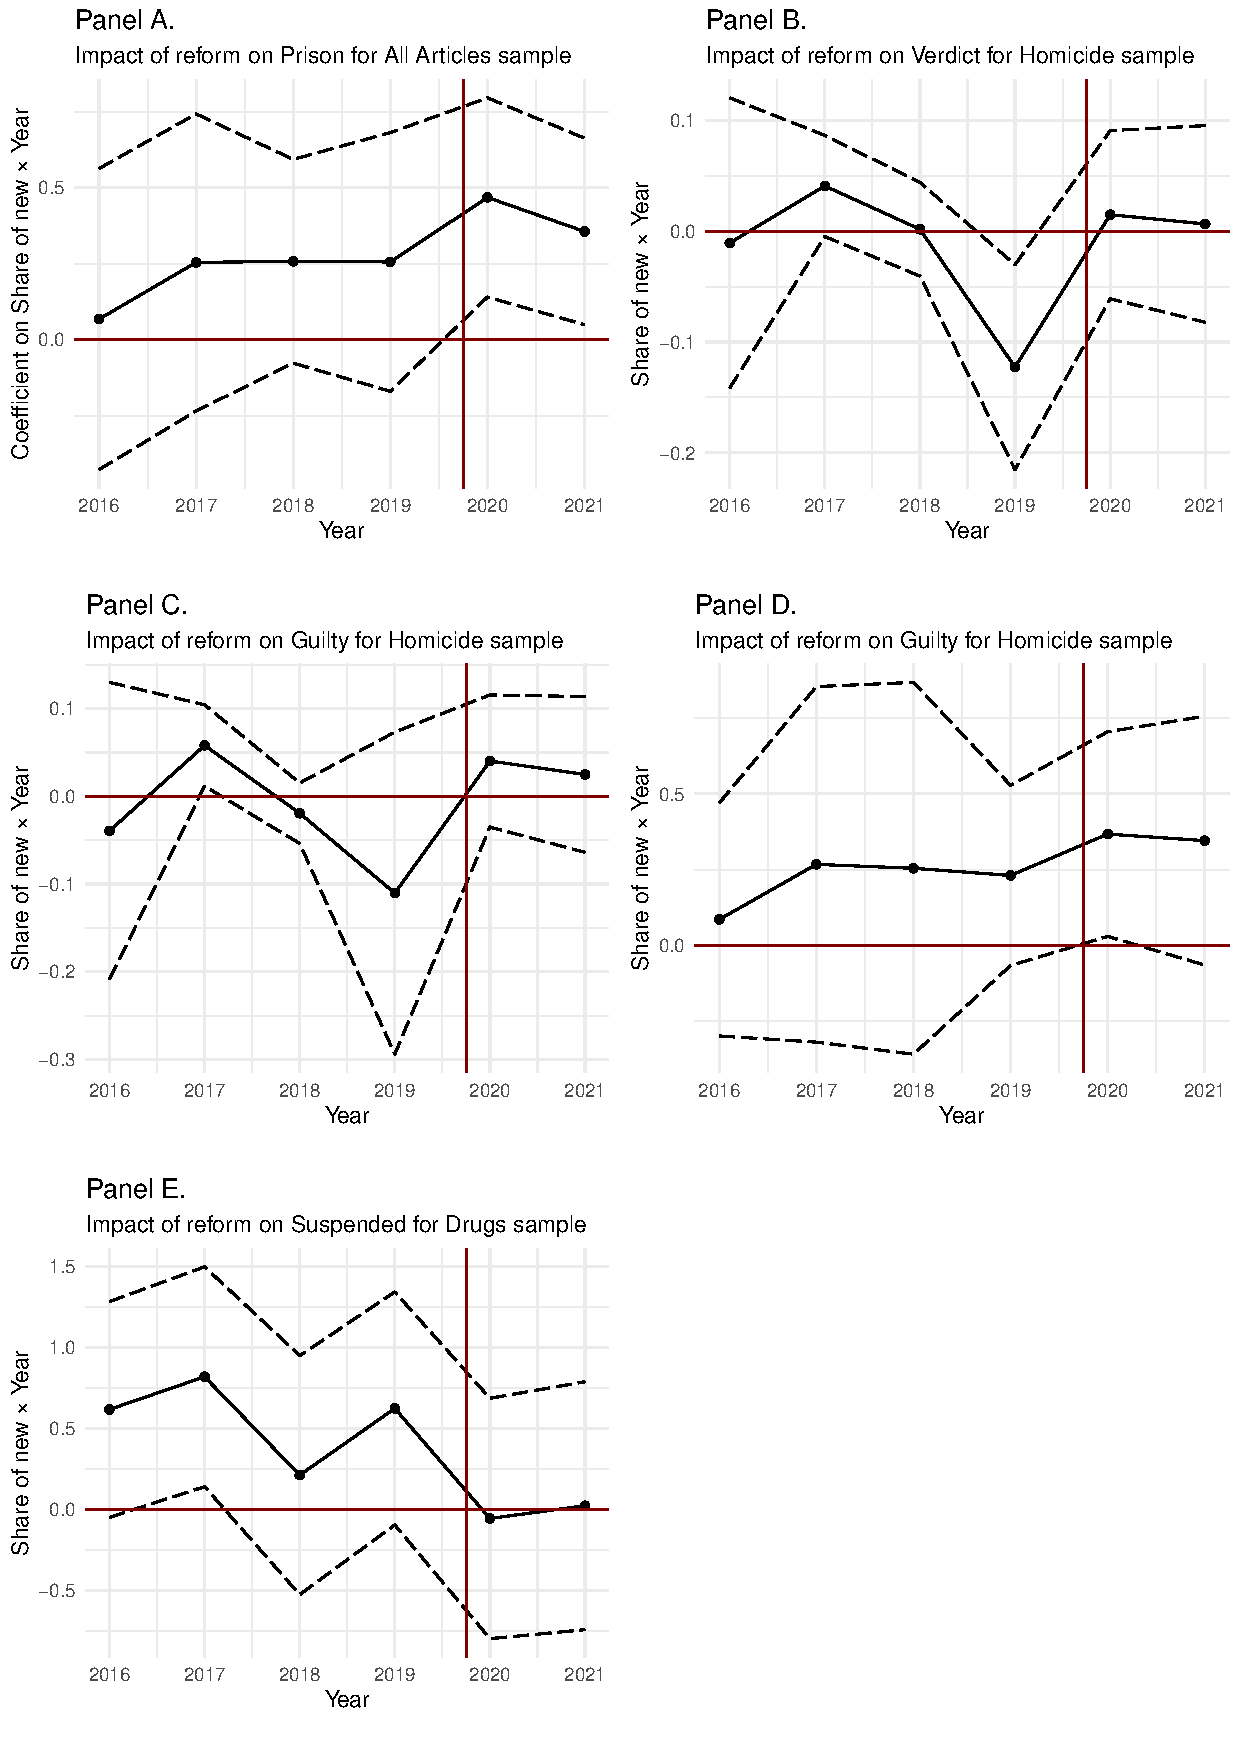
\includegraphics[width=\linewidth]{Rplot.pdf}
        {\begin{flushleft}\footnotesize This figures presents the coefficients $\alpha_k$ and 95\% confidence intervals in the \vref{equation:parallel}. We control for length of verdict and instance (first or appeal) and region-year fixed effects. Errors are two-way clustered on region-year level. \end{flushleft}}
        \end{minipage}
\end{figure}

\section{Discussion of the Results}

The result seems to contradictive. The newly appointed judges give more lenient sentences on average, but the higher the share of newly appointed judges the harsher sentences this court produces. 
It seems that the court that had a larger share of ``treated'' judges began to hand down harsher sentences what contradicts the fact that new judges, on average, make more lenient decisions. 
But since the court chairmen has retained their ability to redistribute judicial proceedings it is possible that the effect of appointment of treated judges is reversed because of that. 


% \section{Conclusion}

\newpage
\references


\newpage
\appendix 

\section{Appendix}
tba

\end{document}